\documentclass[11pt,a4paper]{article}
\usepackage[margin=2.5cm]{geometry}
\usepackage{amsmath,amssymb}
\usepackage{graphicx}
\usepackage{hyperref}

\newcommand{\R}{\mathbb{R}}
\newcommand{\E}{\mathbb{E}}
\newcommand{\norm}[1]{\left\| #1 \right\|}
\newcommand{\ip}[2]{\left\langle #1, #2 \right\rangle}
\newcommand{\xs}{x^\star}

\title{Homework 28.10.26 -- Exercises 29--30}
\author{Gor Melkumyan}
\date{}

\begin{document}
\maketitle

\section*{Exercise 29}

Let $f = \frac{1}{n}\sum_{i=1}^n f_i$, and assume that each $f_i$ is convex and $L_i$-smooth.
Define a gradient estimator by setting $g(x) = \nabla f_i(x)$, where the index $i$ is chosen
uniformly at random. Establish a bound of the form
\[
  G(x,y) \le 2A\,D_f(x,y) + C,
\]
and specify what $A$ and $C$ are. Use this to derive a convergence result for SGD using this
gradient estimator.

\subsection*{Proof}
By the definition of $G(x,y)$ and the fact that $i \sim \mathrm{Uniform}(\{1,2,\dots,n\})$,
\[
  G(x,y) = \E_i\bigl[\norm{g(x) - \nabla f(y)}^2\bigr]
  = \frac{1}{n}\sum_{i=1}^n \norm{\nabla f_i(x) - \nabla f(y)}^2 .
\]
Using $\norm{a+b}^2 \le 2\norm{a}^2 + 2\norm{b}^2$ (Exercise 24) we get
\begin{align*}
  G(x,y)
  &= \frac{1}{n}\sum_{i=1}^n \norm{\bigl(\nabla f_i(x) - \nabla f_i(y)\bigr) + \bigl(\nabla f_i(y) - \nabla f(y)\bigr)}^2 \\
  &\le \frac{2}{n}\left(\sum_{i=1}^n \norm{\nabla f_i(x) - \nabla f_i(y)}^2
     + \sum_{i=1}^n \norm{\nabla f_i(y) - \nabla f(y)}^2\right).
\end{align*}
Since each $f_i$ is convex and $L_i$-smooth, we have
$\norm{\nabla f_i(x) - \nabla f_i(y)}^2 \le 2L_i\,D_{f_i}(x,y)$. Hence, with
$L_{\max} := \max_i L_i$,
\begin{align*}
  G(x,y)
  &\le \frac{4}{n}\sum_{i=1}^n L_i\,D_{f_i}(x,y) + \frac{2}{n}\sum_{i=1}^n \norm{\nabla f_i(y) - \nabla f(y)}^2 \\
  &\le 4L_{\max}\cdot\frac{1}{n}\sum_{i=1}^n D_{f_i}(x,y) + \frac{2}{n}\sum_{i=1}^n \norm{\nabla f_i(y) - \nabla f(y)}^2 \\
  &= 2\,(2L_{\max})\,D_f(x,y) + C(y),
\end{align*}
where we used $D_{f_i}(x,y) \ge 0$ (convexity of $f_i$), the linearity
$D_f = \frac{1}{n}\sum_{i=1}^n D_{f_i}$, and
\[
  C(y) := \frac{2}{n}\sum_{i=1}^n \norm{\nabla f_i(y) - \nabla f(y)}^2 = 2\,\mathrm{Var}\bigl[g(y)\bigr].
\]
As a result, we get
\[
  A = 2L_{\max}, \qquad C = C(y) = \frac{2}{n}\sum_{i=1}^n \norm{\nabla f_i(y) - \nabla f(y)}^2 .
\]

\subsection*{Convergence of SGD}
First of all, it is easy to notice that the estimator is unbiased:
\[
  \E_i\bigl[g(x)\bigr] = \frac{1}{n}\sum_{i=1}^n \nabla f_i(x) = \nabla f(x).
\]
Abd if we take $x = x^k$ and $y = \xs$ in the bound above, and use the fact that 
$\nabla f(\xs) = 0$, then we get
\[
  G^k = \E\bigl[\norm{g^k - \nabla f(\xs)}^2 \,\big|\, x^k\bigr]
  \le 2(2L_{\max})\,D_f(x^k,\xs) + \frac{2}{n}\sum_{i=1}^n \norm{\nabla f_i(\xs)}^2,
\]
i.e.\ the AC assumption holds with
\[
  A = 2L_{\max}, \qquad C = 2\sigma_\star^2, \qquad
  \sigma_\star^2 := \frac{1}{n}\sum_{i=1}^n \norm{\nabla f_i(\xs)}^2 .
\]
If in addition $f$ is $\mu$-convex, Theorem 33 gives that for every stepsize
$0 < \gamma \le \frac{1}{2L_{\max}}$ the iterates of SGD satisfy
\[
  \E\bigl[\norm{x^k - \xs}^2\bigr] \le (1-\gamma\mu)^k\norm{x^0 - \xs}^2 + \frac{2\gamma\sigma_\star^2}{\mu} .
\]
So SGD converges linearly up to a neighbourhood of radius $\frac{2\gamma\sigma_\star^2}{\mu}$,
which shrinks as $\gamma \to 0$. In particular, if $\nabla f_i(\xs) = 0$ for all $i$
(interpolation), then $C = 0$ and SGD converges linearly to $\xs$.

\section*{Exercise 30 (Code)}

Code up the SGD method described in the previous example on an optimization problem of your
choice. Perform a sequence of numerical experiments testing various parts of the established
theory.

\subsection*{What we have to do}
We have to implement SGD
\[
  x^{k+1} = x^k - \gamma\nabla f_{i_k}(x^k), \qquad i_k \sim \mathrm{Uniform}(\{1,\dots,n\}),
\]
with the gradient estimator from Exercise 29, and check numerically what Theorem 33 together
with Exercise 29 predicts:
\begin{enumerate}
  \item for $0 < \gamma \le \frac{1}{A} = \frac{1}{2L_{\max}}$ we have
    $\E\bigl[\norm{x^k - \xs}^2\bigr] \le (1-\gamma\mu)^k\norm{x^0 - \xs}^2 + \frac{\gamma C}{\mu}$;
  \item SGD converges linearly only up to a neighbourhood whose radius is proportional to $\gamma$.
\end{enumerate}

\subsection*{The problem}
We take $n = 12$ one-dimensional quadratics
\[
  f_i(x) = a_i x^2 + b_i x, \qquad f = \frac{1}{12}\sum_{i=1}^{12} f_i .
\]
We do not add constant terms $c_i$ (i.e.\ we take $c_i = 0$), because a constant changes neither
the gradients nor the minimiser, so it plays no role in the minimisation.

The coefficients are just numbers that we generate; there is nothing mathematically important
about them. We only want easy numbers and easy functions that are simple to analyse. We take
random integers $a_i \in \{1,\dots,20\}$ and $b_i \in \{-20,\dots,20\}$ (seed $0$):
\begin{align*}
  a &= (18, 13, 11, 6, 7, 1, 2, 1, 4, 17, 13, 19), \\
  b &= (0, 4, 19, 9, 5, 2, 2, 18, -9, 13, 7, -20).
\end{align*}

For such functions every quantity of the theory can be computed by hand. Let
$\bar a := \frac{1}{n}\sum_i a_i$ and $\bar b := \frac{1}{n}\sum_i b_i$, so that
$f(x) = \bar a x^2 + \bar b x$.

\paragraph{Smoothness.} Since $f_i'(x) = 2a_i x + b_i$, we have
$|f_i'(x) - f_i'(y)| = 2a_i|x-y|$, so $f_i$ is $L_i$-smooth with $L_i = 2a_i$, and
\[
  L_{\max} = 2\max_i a_i, \qquad A = 2L_{\max} = 4\max_i a_i .
\]
Each $f_i$ is convex because $f_i'' = 2a_i > 0$.

\paragraph{Strong convexity.} $f''(x) = 2\bar a$, hence $f$ is $\mu$-convex with $\mu = 2\bar a$.

\paragraph{The minimiser.} $f'(x) = 2\bar a x + \bar b = 0$ gives
\[
  \xs = -\frac{\bar b}{2\bar a} = -\frac{\sum_i b_i}{2\sum_i a_i} .
\]

\paragraph{The constant $C$.} From Exercise 29, $C = 2\sigma_\star^2$ where
$\sigma_\star^2 = \frac{1}{n}\sum_i |f_i'(\xs)|^2$, and $f_i'(\xs) = 2a_i\xs + b_i$, so we get
\[
  C = \frac{2}{n}\sum_{i=1}^n \bigl(2a_i\xs + b_i\bigr)^2 .
\]

\paragraph{Our numbers.} $\sum_i a_i = 112$, $\sum_i b_i = 50$ and $\max_i a_i = 19$, so
\begin{gather*}
  \xs = -\tfrac{50}{224} = -\tfrac{25}{112} \approx -0.2232, \qquad
  \mu = \tfrac{112}{6} = \tfrac{56}{3} \approx 18.67, \\
  L_{\max} = 38, \qquad A = 76, \qquad C \approx 263.31 .
\end{gather*}
We start from $x^0 = 10$ and estimate $\E\bigl[\norm{x^k - \xs}^2\bigr]$ by averaging over
$2000$ independent runs of SGD.

The code is the file
\href{https://github.com/Gor-2001/thesis_hw/blob/main/Homework/Exercises/hw_2026_10_28/ex30_sgd.ipynb}{\texttt{Homework/Exercises/hw\_2026\_10\_28/ex30\_sgd.ipynb}}.

\subsection*{Experiment 1: the bound of Theorem 33}
We take the largest stepsize allowed by the theory, $\gamma = \frac{1}{A} = \frac{1}{76}$.

\begin{center}
  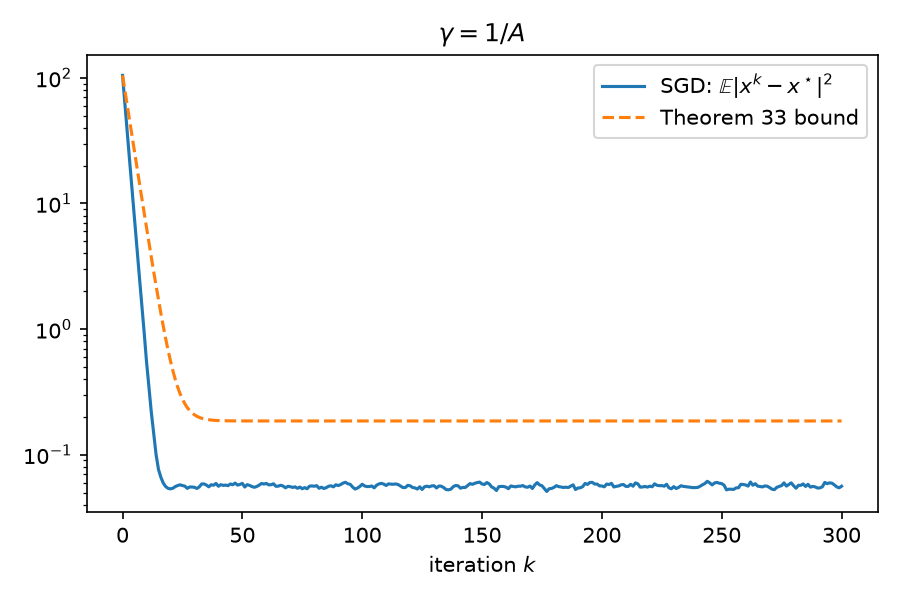
\includegraphics[width=0.7\textwidth]{figures/exp1_bound.png}
\end{center}

The error decreases linearly and then stays at about $5.6\cdot 10^{-2}$. The bound is never
violated, and its limit is $\frac{\gamma C}{\mu} \approx 0.186$.

\subsection*{Experiment 2: the neighbourhood is proportional to $\gamma$}
We take $\gamma = \frac{1}{mA}$ for $m = 1, 4, 16, 64$ (dashed lines: $\frac{\gamma C}{\mu}$).

\begin{center}
  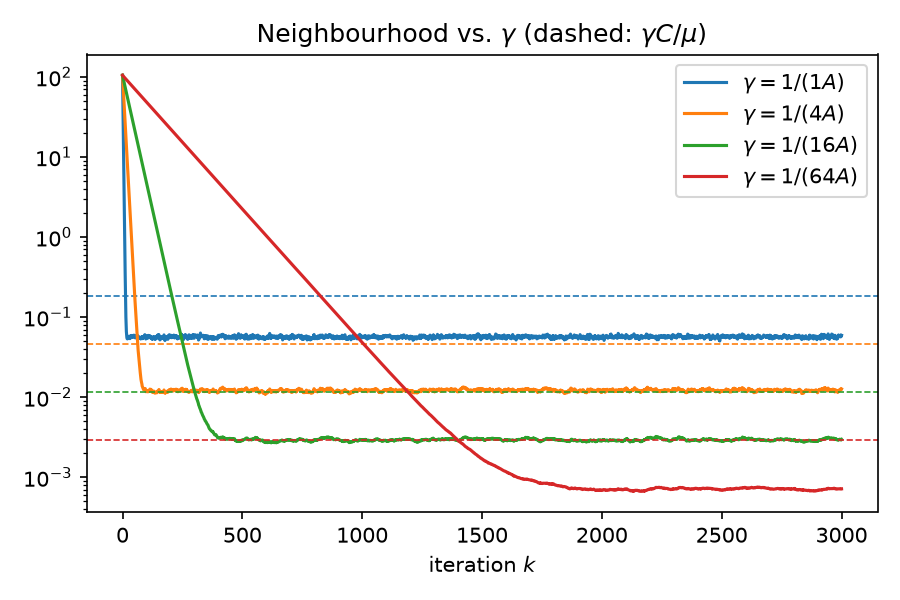
\includegraphics[width=0.7\textwidth]{figures/exp2_neighbourhood.png}
\end{center}

\begin{center}
\begin{tabular}{cccc}
  $\gamma$ & plateau (SGD) & exact limit & $\gamma C/\mu$ \\ \hline
  $1/A$    & $5.67\cdot 10^{-2}$ & $5.67\cdot 10^{-2}$ & $1.86\cdot 10^{-1}$ \\
  $1/(4A)$ & $1.22\cdot 10^{-2}$ & $1.22\cdot 10^{-2}$ & $4.64\cdot 10^{-2}$ \\
  $1/(16A)$ & $2.94\cdot 10^{-3}$ & $2.93\cdot 10^{-3}$ & $1.16\cdot 10^{-2}$ \\
  $1/(64A)$ & $7.16\cdot 10^{-4}$ & $7.27\cdot 10^{-4}$ & $2.90\cdot 10^{-3}$
\end{tabular}
\end{center}

Dividing $\gamma$ by $4$ divides the plateau by about $4$, as predicted. The price is a slower
linear rate $1-\gamma\mu$. The plateau agrees with the exact formula, and the ratio
plateau$/(\gamma C/\mu)$ tends to $\frac{1}{4}$.
\end{document}
